\documentclass[11pt]{article}
\usepackage{tikz}
\usepackage{fullpage}
\usepackage{algorithm}
\usepackage[noend]{algorithmic}
\usepackage{enumerate}
\usepackage{amsmath,amssymb,amsthm}
\usepackage{stackrel}

\usepackage{multicol}
\usepackage{lipsum}% dummy text

\setlength{\columnseprule}{0.4pt}


% Helpful Shortcuts
\newcommand{\bc}[1]{{\quad \text{(#1)}}} 	% Justification in math env
\newcommand{\st}{{\text{ such that }}} 							   % Math env
\newcommand{\abs}[1]{{ |#1 |}} 							% Absolute value / Cardinality
\newcommand{\bld}[2]{\noindent\textbf{#1:}\hspace{0.1in}#2$  $\bigskip} % Headings
\newcommand{\notimplies}{%
	\mathrel{{\ooalign{\hidewidth$\not\phantom{=}$\hidewidth\cr$\implies$}}}}
\newcommand{\linesep}{\noindent\bigskip\rule{17cm}{0.1mm}\bigskip} % Horizontal Line

% These define new environments / formats for lemmas, definitions, running time, etc.
\newtheorem{lemma}{Lemma}
\newtheorem{definition}{Definition}
\newtheorem{notation}{Notation}
\newtheorem*{claim}{Claim}
\newtheorem{observation}{Observation}
\newtheorem{conjecture}[lemma]{Conjecture}
\newtheorem{theorem}[lemma]{Theorem}
\newtheorem{corollary}[lemma]{Corollary}
\newtheorem{proposition}[lemma]{Proposition}
\newtheorem*{rt}{Running Time}

% These define nice ways to format P and OPT (use \P or \opt)
\def\P{\ensuremath{$ \mathcal{P} $}}
\def\opt{\ensuremath{\textsc{opt}}}
\renewcommand{\labelenumi}{\bf \alph{enumi}.}

\renewcommand\maketitle{
	\begin{center}
		\begin{tabular*}{6.44in}{l @{\extracolsep{\fill}}c r}
			\bfseries  &  & \bfseries CSCI 383 Spring 2019 \\
			\bfseries&  & \bfseries  Homework \#9 Solutions  \\
			\bfseries   &   &  \bfseries Kai Ting Keshia Yap\\ 
		\end{tabular*}
\end{center} }

\begin{document}
	\maketitle
	
	\noindent Honor Code: I affirm that I adhered to the Honor Code in this assignment. Keshia Yap\\
	
	
	\subsection*{Part 3: Large Front Teeth}
	This question explores the workings of the infamous busy beaver problem. Given a number k, one
	must build a special beaver-driven Turing machine. This machine has a two-way infinite tape, tape
	alphabet $ \Gamma = \{1, t\}, k $ normal states and one halting state. The goal is to construct a machine
	that, upon starting with a blank tape, writes as many 1s on the tape as possible before halting. We
	define the busy beaver function $ BB : N \rightarrow N $ such that $ BB(k) $ is the maximum number of 1s that
	remain on the tape among all of these special Turing machines with k normal states. For example, we know that $ BB(1) = 1 $.\\
	
	That is, if we start with a blank tape, the above TM is able to write out six 1’s before halting. It turns out that if a beaver is in charge of writing down all these 1s, then he is a busy beaver indeed. The busy beaver function was first defined by Tibor Rados, in a 1962 paper. Since then, the only known $ BB(k) $’s are for $ k \leq 4 $. In fact, it grows faster than any computable function! Some known lower bounds are that $ BB(5) \geq4, 098 $, $ BB(6) \geq 4.6 \times 101439 $, and $ BB(10) > 3^{3^{3^{.^{.^{.^{3}}}}}} $, where there are 327 terms in the exponential tower. Seriously.
	\linesep
	\begin{enumerate}
		\item Show the sequence of 15 configurations of the $ k = 3 $ machine, to prove that it actually outputs 6 ones. Your first configuration should be $ (s, \underline{\textvisiblespace}\:\textvisiblespace\:\textvisiblespace) $ and your final configuration should be $ (h, 111111) $.

		\textbf{Configurations:}
			\begin{multicols}{4}
				\begin{center}
					\begin{enumerate}[1.]
					\item $ (s, \underline{\textvisiblespace}\:\textvisiblespace\:\textvisiblespace)  $\\
					\item $ (u, 1\:\underline{\textvisiblespace}\:\textvisiblespace)  $\\
					\item $ (v, 1\:\textvisiblespace\:\underline{\textvisiblespace})  $\\
					\item $ (v, 1\:\underline{\textvisiblespace}\:1)  $\\
					\item $ (v, \underline{1}\:\textvisiblespace\:1)  $\\
					\item $ (s, \underline{\textvisiblespace}1\:\textvisiblespace\:1)  $\\
					\item $ (u, 1\:\underline{1}\:\textvisiblespace\:1)  $\\
					\item $ (u, 1\:1\:\underline{\textvisiblespace}\:1)  $\\
					\item $ (v, 1\:1\:\textvisiblespace\:\underline{1})  $\\
					\item $ (s, 1\:1\:\underline{\textvisiblespace}\:1)  $\\
					\item $ (u, 1\:1\:1\:\underline{1})  $\\
					\item $ (u, 1\:1\:1\:1\:\underline{\textvisiblespace})  $\\
					\item $ (v, 1\:1\:1\:1\:\textvisiblespace\:\underline{\textvisiblespace})  $\\
					\item $ (v, 1\:1\:1\:1\:\underline{\textvisiblespace}\:1)  $\\
					\item $ (v, 1\:1\:1\:\underline{1}\:1\:1)  $\\
					\item $ (s, 1\:1\:\underline{1}\:1\:1\:1)  $\\
					\item $ (h, 1\:1\:1\:\underline{1}\:1\:1)  $\\
				\end{enumerate}
				\end{center}
			\end{multicols}

		\item Show that $ BB(2) \geq 4  $ by constructing a 3-state TM with one halting state such that, when started with an empty tape, your TM produces four 1’s.
			\begin{center}
				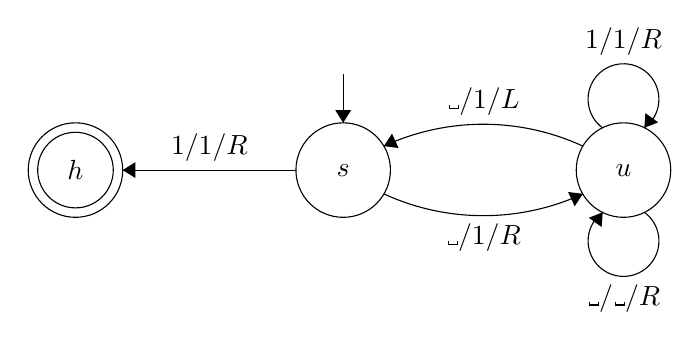
\begin{tikzpicture}[scale=0.2]
				\tikzstyle{every node}+=[inner sep=0pt]
				\draw [black] (23.3,-26.6) circle (3);
				\draw (23.3,-26.6) node {$s$};
				\draw [black] (6.3,-26.6) circle (3);
				\draw (6.3,-26.6) node {$h$};
				\draw [black] (6.3,-26.6) circle (2.4);
				\draw [black] (41.1,-26.6) circle (3);
				\draw (41.1,-26.6) node {$u$};
				\draw [black] (20.3,-26.6) -- (9.3,-26.6);
				\fill [black] (9.3,-26.6) -- (10.1,-27.1) -- (10.1,-26.1);
				\draw (14.8,-26.1) node [above] {$1/1/R$};
				\draw [black] (38.516,-28.114) arc (-65.3223:-114.6777:15.127);
				\fill [black] (38.52,-28.11) -- (37.58,-27.99) -- (38,-28.9);
				\draw (32.2,-30) node [below] {$\textvisiblespace/1/R$};
				\draw [black] (23.3,-20.5) -- (23.3,-23.6);
				\fill [black] (23.3,-23.6) -- (23.8,-22.8) -- (22.8,-22.8);
				\draw [black] (39.777,-23.92) arc (234:-54:2.25);
				\draw (41.1,-19.35) node [above] {$1/1/R$};
				\fill [black] (42.42,-23.92) -- (43.3,-23.57) -- (42.49,-22.98);
				\draw [black] (42.423,-29.28) arc (54:-234:2.25);
				\draw (41.1,-33.85) node [below] {$\textvisiblespace/\textvisiblespace/R$};
				\fill [black] (39.78,-29.28) -- (38.9,-29.63) -- (39.71,-30.22);
				\draw [black] (25.88,-25.079) arc (114.80737:65.19263:15.062);
				\fill [black] (25.88,-25.08) -- (26.82,-25.2) -- (26.4,-24.29);
				\draw (32.2,-23.19) node [above] {$\textvisiblespace/1/L$};
				\end{tikzpicture}
			\end{center}
		\textbf{Configurations:}
		\begin{multicols}{2}
			\begin{enumerate}[1.]
				\item $ (s,\underline{\textvisiblespace}\:\textvisiblespace\:\textvisiblespace\:\textvisiblespace) $
				\item $ (u,1\:\underline{\textvisiblespace}\:\textvisiblespace\:\textvisiblespace) $
				\item $ (u,1\:\textvisiblespace\:\underline{\textvisiblespace}\:\textvisiblespace) $
				\item $ (s,1\:\underline{\textvisiblespace}\:1\:\textvisiblespace) $
				\item $ (u,1\:1\:\underline{1}\:\textvisiblespace) $
				\item $ (u,1\:1\:1\:\underline{\textvisiblespace}) $
				\item $ (s,1\:1\:\underline{1}\:1) $
				\item $ (h,1\:1\:1\:\underline{1}) $
			\end{enumerate}
		\end{multicols}
		\item  Show that $ BB $ is not a computable function (that is, there is no TM that takes as input a
		number $ k $ in unary and halts with $ BB(k) $ written on the tape).
	Hint: Use $ BB(k) $ to solve the halting problem. Have it help you remember how many steps
	it takes M to halt on $ x $ and use this information to your advantage.’
	
	\linesep
	
	Let $ M^* $ be a Turing machine that accepts $ k\#BB(k) $. Let $ K $ be the Turing machine with input $ N\# x $ given $ M^*$ and the reduction $ R $ where $ K $ accepts $ N\#x $ if and only if $ M^* $ accepts the output of $ R $. Let $ R $ run the following algorithm:
	\begin{algorithm}
	\begin{algorithmic}
		\STATE Run $ N $ on $ x $
		\IF{$ N $ halts on $ x $}
		\RETURN{$ k\#BB(k) $ where $ k $ is the number of steps that $ N $ took to halt on $ x $.}
		\ELSE
		\RETURN{$ 0 $}
		\ENDIF
	\end{algorithmic}
	\end{algorithm}\\

	This shows that $ x\in L(N) $ if and only if we found $ BB(k) $, solving the membership problem which is not computable. So $ BB $ is not a computable function.
	\end{enumerate} 
\end{document}